\chapter{Evaluation}
\label{sec:evaluation}
% TODO: Segmentation als Metrik
Im Kapitel Evaluation werden die im Kapitel 5 vorgestellten Experimenten evaluiert. Außerdem wird die gewählte Methode ausgewertet und
mit andere Methoden verglichen.

\section{Evaluationsmetrik}
Für das Problem von Image colorization existiert keine relevante Evaluationsmetrik die die Farben von dem Objekten auf einem Bild auswerten kann.
Das während das Training angewendete Cross Entropy Loss ist nicht relevant für die Auswertung der Ergebnisse aus dem Test Datensatz. Aus diesem
Grund wurde die Evaluation der Ergebnisse durch eine Menschliche Auswertung wie bei \cite{zhang2016colorful} und \cite{billaut2018colorunet}
durchgeführt.

\section{Evaluation des Spiel-Datensatzes}
Mit dem Spiel-Datensatz wurde die Funktionsweise der Methode bestätigt. Die von Billaut et al. vorgeschlagene Netzwerkarchitektur für Image
colorization hat beeindruckende Ergebnissen mit wenige Epochen erreicht. 
\\
Die gewählte Methode für das Binning funktionierte und hat ermöglicht die Originale Farben wiederherzustellen. Die Anzahl an 
Bins war für diesen Datensatz nicht relevant da es nur 9 gleich möglichen Farben gab.

\begin{figure}[H]
  \vspace{1cm}
  \centering
  \begin{subfigure}
    \centering
    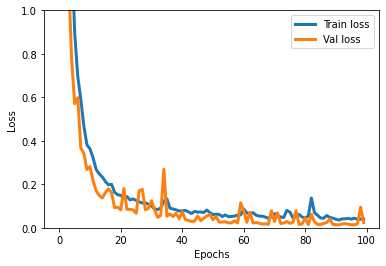
\includegraphics[width=.5\textwidth]{resources/experiments/toy_100_324_0001.png}
  \end{subfigure}
  \caption{Training und Validation Loss Verlauf von dem Spiel-Datensatz}
  \label{image:toy-dataset-loss}
\end{figure}

\section{Evaluation des CIFAR-100 Subsets}
Die Ergebnissen aus dem CIFAR-100 Subset zeigten dass das Model in wenige Epochen viele Merkmale lernen konnte. Ein wichtiger Faktor zu 
erwähnen ist dass die Gewichte des Netzwerks zufällig initialisiert wurden und nicht vortrainiert waren. 
\\
\\
Auf diesem Datensatz wurde die Auswirkung der Bin Anzahl gemessen. Die Auswahl von 36 Bins zeigten im Vergleich zu 324 eine 
Verschlechterung der Farben in der Vorhersage. Dies ist darauf zurückzuführen dass das Model nur 36 mögliche Farben zu Verfügung hat.
Eine Erhöhung der Bins auf 324, ermöglichte das Model eine Auswahl an mehr Farben zu treffen. 
Den Ansatz von \cite{billaut2018colorunet} verwendet nur 32 Bins und erzielt ähnliche Ergebnisse wie die Methode dieser Arbeit mit 324 Bins.
Dies wurde erreicht in dem die Pixeln von jedem Trainingsbild vor dem Training in Bins klassifiziert wurden und daraus nur die am meisten
vorkommenden 32 Bins ausgewählt wurden. Pixeln die nicht in den gewählten 32 Bins klassifiziert werden konnten, wurden in das nächstliegende Bin
zugeordnet.
\\
\\
Der Methode mit einem MSE Loss ermöglicht eine um ein vielfaches größere Auswahl an Farben für die Vorhersage. Bei dieser Methode tretten 
die im Kapitel \ref{subsection:verwandte-arbeiten} erwähnten Schwierigkeiten, wobei in dem Fall von diesem Datensatz, diese Schwierigkeiten
kaum zu erkennen waren.
Da die Klassifikationsmethode leicht bessere Ergebnissen geliefert hat und der Fokus der Arbeit auf Klassifikationsmethoden gesetzt war,
wurden alle Experimenten des Landscape Datensatzes mit der Klassifikationsmethode durchgeführt.
\\
\\
Der Verlauf von dem Training und Validation Loss deutete bei diesem Datensatz zu overfitting, was bei der Große des Datensatzes nicht auszuschließen war.
Wie bei \ref{section:cifar-experimente} beschrieben wurden das U-net und die Hyperparameter angepasst um dieses zu verhindern.

\begin{figure}[H]
  \centering
  \vspace{1cm}
  \begin{subfigure}
    \centering
    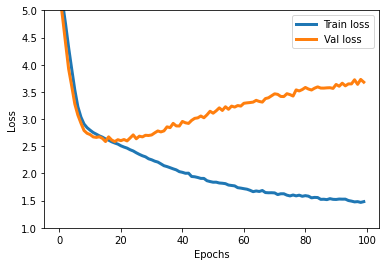
\includegraphics[width=.48\textwidth]{resources/experiments/cifar_100_324_0001.png}
  \end{subfigure}
  \begin{subfigure}
    \centering
    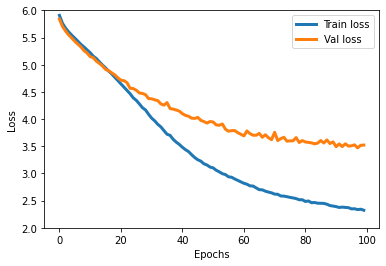
\includegraphics[width=.48\textwidth]{resources/experiments/cifar_100_324_00001.png}
  \end{subfigure}

  \caption{Overfitting auf dem CIFAR-100 Subset. \textbf{Links}: 100 Epochen mit Adam, ReLU und eine Lernrate von 0.001. \textbf{Rechts}:
  100 Epochen mit Adam, ReLU und eine Lernrate von 0.0001.}
  \label{image:gute-ergebnisse-cifar}
\end{figure}

Eine Anpassung der Lernrate führte nur zu einem langsameres Training. Eine Reduktion der lernbare Parameter von 135684 auf 35748 zeigte 
eine deutliche Verbesserung der Performance des Models und reduzierte das Overfitting.

\begin{figure}[H]
  \centering
  \vspace{1cm}
  \begin{subfigure}
    \centering
    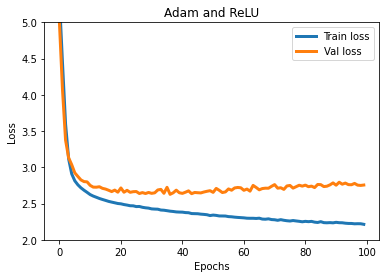
\includegraphics[width=.48\textwidth]{resources/experiments/cifar-adam-relu.png}
  \end{subfigure}
  \begin{subfigure}
    \centering
    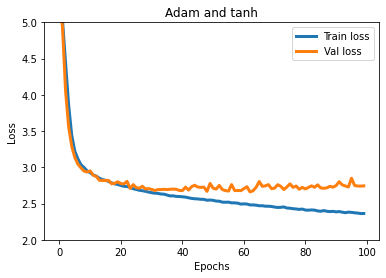
\includegraphics[width=.48\textwidth]{resources/experiments/cifar-adam-tanh-100.png}
  \end{subfigure}

  \caption{Loss Verlauf mit eine reduzierte Anzahl an Parameter und verschiedene Aktivierungsfunktionen. 
  \textbf{Links}: 100 Epochen mit Adam, ReLU und eine Lernrate von 0.001. \textbf{Rechts}: 100 Epochen mit Adam, Tanh und eine Lernrate von 0.001.}
  \label{image:gute-ergebnisse-cifar}
\end{figure}

Der Grund für das Overfitting ist in diesem Fall zu der Große des Subsets zurückzuführen. Um das zu prüfen wurde das Model auf das komplette CIFAR-100
Datensatz für 150 Epochen trainiert, was einen guten Loss Verlauf zeigte. Auf der anderen Seite, hat das Model nichts relevantes gelernt und 
konnte kein Bild richtig einfärben, was bei der Anzahl der Klassen und die Anzahl der Epochen normal ist.

\section{Evaluation des Landscape Datensatzes}
Die Ergebnisse dieses Model zeigen dass die ausgewählte Methode, mit wenige Bildexemplare und Epochen, sehr gute Ergebnisse erreichen kann.
Die Anzahl der Bins für diesen Datensatz wurde durch die vorgeführten Experimenten auf 324 gesetzt, da dieser Anzahl die beste Kombination
aus Trainingszeit und Performance erwiesen hat.
\\
\\
Der Loss Verlauf der Experimenten deutete ebenfalls bei diesem Datensatz nach wenige Epochen auf Overfitting. Nach Zahlreichen Experimenten
konnte das Overfitting durch Anpassung der Hyperparameter nur minimiert werden. Für die Auswertung der Ergebnissen wurde das Model mit den besten
Validation Loss verwendet.
\\
\\
Bei der Evaluation der Ergebnissen ist zu erkennen dass nach den wenigen Epochen das Model die wichtigsten Entitäten wie der Himmel, Wolken, Wasser,
Grass und Erde richtig Einfärben kann. Es fällt auf dass bei einigen Bildern, die Vorhersage des Models realer aussieht als das Originale Bild
wie das zweite Beispiel von \ref{image:gute-ergebnisse-own}. Im Vergleich zu das Model von \cite{billaut2018colorunet} sehen die vorhergesagten 
Farben von dieses Model sehr ähnlich. Das zeigt die Performance der Methode ohne die Optimierungstechniken die bei \cite{billaut2018colorunet}
angewendet wurden. Die Auswirkung der Temperaturwert ist auf beiden Modellen ähnlich, den Modus der Verteilung zeigt einen rötlichen Ton bei den
Ergebnissen und den Durchschnitt zeigt bei einigen Fällen gesättigte Bilder.
\\
Da die Datensatz Große von \cite{billaut2018colorunet} fast identisch ist zu der Datensatz Große dieser Arbeit, konnte das Problem mit dem Overfitting
auf die Qualität des Datensatzes zurückzuführen sein. Deren Loss Verlauf zeigt kein Overfitting und das verwendete U-Net ist sehr ähnlich wie das
U-Net der vorliegende Arbeit, was ein Overfitting wegen der angewendete Netzwerkarchitektur ausschließt.
\\
\\
Ein Vergleich mit den Ergebnissen von \cite{zhang2016colorful} wär nur fair mit den Ergebnissen aus deren Klassifikationsmodell ohne rebalancing.
In diesem Fall sind die Ergebnissen dieses Modells nicht weit entfernt von deren Ergebnissen. Es ist zu erkennen dass deren Modell die gleiche 
Probleme zeigt wie das Model dieser Arbeit. 
% Die Ergebnissen von \cite{zhang2016colorful} zeigen bei den meisten Bildern eine bessere Farbe Vorhersage im Vergleich zu die Vorhersagen dieses
% Models.



% Beispiel einer Tabelle:
% \begin{longtable}{|c|c|c|c|}
% 	\hline
% 	\multicolumn{1}{|c}{\textbf{Spalte 1}} &
% 	\multicolumn{1}{|c}{\textbf{Spalte 2}} &
% 	\multicolumn{1}{|c|}{\textbf{Spalte 3}} \\
% 	\hline
% 	\endfirsthead
	
% 	\multicolumn{3}{c}{Beschreibung}\\ \hline
% 	\multicolumn{1}{|c}{\textbf{Spalte 1}} &
% 	\multicolumn{1}{|c}{\textbf{Spalte 2}} &
% 	\multicolumn{1}{|c|}{\textbf{Spalte 3}} \\
% 	\hline
% 	\endhead
	
% 	\multicolumn{2}{c}{Fortsetzugn auf der nächsten Seite}
% 	\endfoot
	
% 	\caption{Beschreibung}
% 	\label{tab:example}
% 	\endlastfoot
	
% 	TODO & TODO & TODO \\ \hline
% 	TODO & TODO & TODO  \\ \hline
% \end{longtable}

% \section{Beispiel Unterkapitel}
% TODO